\newpage
\section{Configuration Syntax}
%        --------------------
\subsection{Conventions}
%           -----------
%%%%%%%%%%%%%%%%%%%%%%%%%%%%%%%%%%%%%%%%%%%%%%%%%%%%%%%%%%%%%%%%%%%%%%%%%%%%%
%%%                               Syntax                                  %%%
%%%%%%%%%%%%%%%%%%%%%%%%%%%%%%%%%%%%%%%%%%%%%%%%%%%%%%%%%%%%%%%%%%%%%%%%%%%%%
\index{Conventions}
The parser reads and interpretes
the configuration data file to configure the \INTENS{} application
at each program startup.
This section describes the syntax of the \INTENS{} script (configuration) language.

The following conventions are used in the syntax diagrams:
\vspace{1cm}

\begin{figure}[h]\label{fig:syntaxConventions}
  \begin{center}
    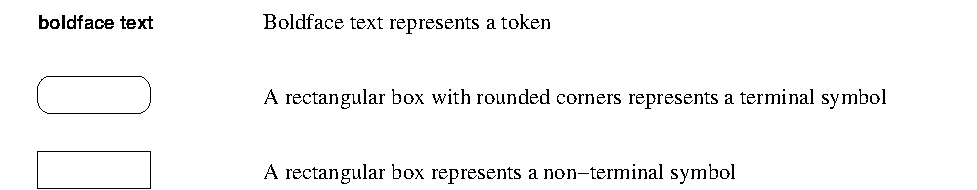
\includegraphics[width=\linewidth]{xfig/sntx_conventions}
  \end{center}
  \caption{Syntax conventions}
\end{figure}
\vspace{1cm}

\begin{itemize}
\item
Any text is considered to be case sensitive.

\item
Characters after \verb+//+ are ignored. They may be
used as comment marks. \index{Conventions!comment}
\verb+#+-characters can be used for macro definitions
in combination with a pre-compiler.

\item
Floating-point \index{Conventions!floating-point}
constants contain a decimal point (\verb+3.14+) or an exponent (\verb+1e-2+) or both.

\item
A string constant \index{Conventions!string constant}
is a sequence of zero or more characters surrounded by double
quotes.
 Two or more following string constants can be concatenated with an \& operator:
\begin{verbatim}
 "Im Innern der Erde " & "wütet das Nichts."
\end{verbatim}

\item
A string can be composed at parse time (i.E. needed for translation):
\begin{verbatim}
  COMPOSE_STRING("Create new %1.", LABEL(motor))
\end{verbatim}
\end{itemize}
